
% --------------------------------------------------------------------
% This is a simple Beamer document that uses beamerthemesigma.sty
% Reading the comments should help you create a presentation even if
% you've never used Beamer before.
% --------------------------------------------------------------------
% Set our document class to Beamer
\documentclass[aspectratio=169]{beamer}

% Some packages for nice font encodings in the final PDF
\usepackage[utf8]{inputenc}
\usepackage[T1]{fontenc}

% From Jeff E
\usepackage{algo}

\usepackage{sigmastyle}

% To insert images
\usepackage{graphicx}

% Useful packages from the AMS
\usepackage{amsmath,amssymb,amsthm}

% Package for code highlighting
\usepackage{minted}
\setminted{linenos=true, breaklines=true, breakanywhere=true, style=default}
\usemintedstyle{monokai}

% Set a title
\title{Reductions}

% The subtitle is generally where I'd expect you to put the week
% number, thus:
\subtitle{Week 9}
% \texorpdfstring to remove compilation warnings if you have math here

% Whoever worked on the presentation:
\author{Anakin}

% A date, if you'd like.
\date{}

% An institute name, if you're so inclined
% \institute{University of Illinois Urbana-Champaign}

% Use the SIGma theme for this Beamer presentation
\usetheme{sigma}
% --------------------------------------------------------------------
% Begin document
\begin{document}

% Beamer calls each slide a "frame", defined within the environment:
% \begin{frame}
%   <frame content here>
% \end{frame}

% This frame is just the title.
\begin{frame}
\titlepage
\end{frame}

% A frame with the table of contents.
% This frame's title is "Outline".
\begin{frame}{Outline}
  \tableofcontents
\end{frame}

\begin{frame}{Updates!}
  Weekly updates: \pause
  \begin{itemize}
    \item Stickers have been ordered
    \item I'll let everyone know when they get here
  \end{itemize}
\end{frame}

\section{Review}
\frame{\sectionpage}

\begin{frame}{What We Know}
    \begin{itemize}
        \item We say that $M$ \textbf{\textit{recognizes/accepts}} $L$ if for any input $w\in L$, $M$ accepts $w$. \pause
        \begin{itemize}
            \item If $w \in L$, then $M$ must \textbf{accept} $w$
            \item If $w \notin L$, then $M$ can \textbf{reject} or even \textbf{never halt} \pause
        \end{itemize}
        \item $M$ \textbf{\textit{decides}} $L$ if for any input $w$, $M$ accepts if $w \in L$ and rejects otherwise. \pause
        \begin{itemize}
            \item If $w \in L$, then $M$ must \textbf{accept} $w$
            \item If $w \notin L$, then $M$ must \textbf{reject} $w$ \pause
            \item Either way, $M$ must halt on all inputs
        \end{itemize}
    \end{itemize}
\end{frame}

\begin{frame}{What We Know}
    \begin{itemize}
        \item $L$ is \textbf{recognizable} if there exists some TM $M$ that recognizes it \pause
        \item $L$ is \textbf{decidable} if there exists some TM $M$ that decides it \pause
        \item Some languages are unrecognizable or undecidable
    \end{itemize}
\end{frame}

\begin{frame}{Key Examples}
    \begin{itemize}
        \item $HALT_{\text{TM}} = \set{\langle M, w \rangle | \text{$M$ is a TM and $M$ halts on input $w$}}$
        \begin{itemize}
            \item We showed this language is undecidable \pause
        \end{itemize}
        \item $A_{\text{TM}} = \set{\langle M, w \rangle | \text{$M$ is a TM and $M$ accepts $w$}}$ 
        \begin{itemize}
            \item We showed this language is undecidable \pause
        \end{itemize}
        \item $\overline{A_{\text{TM}}} =$ complement of $A_{\text{TM}}$
        \begin{itemize}
            \item We showed this language is unrecognizable
        \end{itemize}
    \end{itemize}
\end{frame}

\begin{frame}{How Do We Figure Out More?}
    \begin{itemize}
        \item The proofs for all of these were long and confusing \pause
        \item What if we wanted to prove other languages are undecidable/unrecognizable? \pause
        \begin{itemize}
            \item Do you want to do all that work again? 
            \item I don't \pause
        \end{itemize}
        \item What if we could leverage our previous proofs?
    \end{itemize}
\end{frame}

\section{Reductions}
\frame{\sectionpage}

\begin{frame}
  \begin{center}
    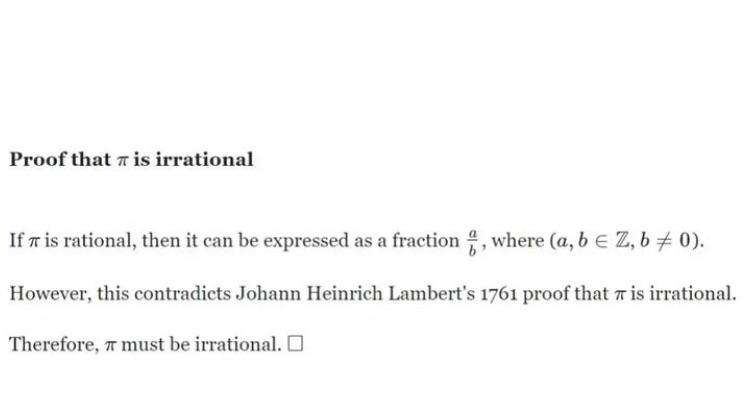
\includegraphics[width=\textwidth]{images/pi_proof.jpg}
  \end{center}
\end{frame}

\begin{frame}{What Is A Reduction?}
    \begin{itemize}
        \item As stupid as it is, the previous proof follows the idea of a reduction \pause
        \item We assume something and reach a conclusion that contradicts a known result, thus proving our assumption was incorrect
    \end{itemize}
\end{frame}

\begin{frame}{What Is A Reduction?}
    \begin{itemize}
        \item A \textbf{decidability} reduction is a proof of the following form: \pause
        \begin{itemize}
            \item Suppose language $L$ is decidable, then there exists a TM $M$ that decides it \pause
            \item We can use $M$ as a blackbox in some other algorithm to decide your favorite undecidable problem \pause
            \item This contradicts the fact that your chosen problem is undecidable \pause
            \item Thus $L$ is undecidable
        \end{itemize}
    \end{itemize}
\end{frame}

\begin{frame}{Reductions = Algorithms}
    \begin{itemize}
        \item This is the format of a \textbf{Turing Reduction}\footnotemark\ \footnotetext{CS 374 talks about mapping reductions, which are equivalent but more confusing} \pause
        \item You are given access to some blackbox oracle \pause
        \begin{itemize}
            \item Imagine the oracle like some library function you import \pause
            \item You know what it takes as input and gives as output \pause
            \item You just don't know exactly how it works \pause
        \end{itemize}
        \item You write an algorithm using this oracle \pause
        \item If you are reducing from $A$ to $B$, then your algorithm should accept \textbf{if and only if} the input is in language $A$
    \end{itemize}
\end{frame}

\begin{frame}{Difficulty}
    \begin{itemize}
        \item Reductions play an extremely central in complexity theory since it allows to talk about how \textbf{hard problems} are \pause
        \item If we can reduce Problem $A$ to Problem $B$, solving $A$ cannot be harder than solving $B$  
        \begin{itemize}
            \item Solving $B$ gives a solution to $A$ \pause
        \end{itemize}
        \item Thus if $A$ reduces to $B$ and we know something about $A$, we learn: \pause
        \begin{itemize}
            \item if $A$ is undecidable, then $B$ is undecidable \pause
            \item if $A$ is unrecognizable, then $B$ is unrecognizable 
        \end{itemize}
    \end{itemize}
\end{frame}

\begin{frame}{Decidability Reduction}
    $$E_{\text{TM}} = \Set{\langle M \rangle | M \text{ is a TM and } L(M) = \emptyset}$$ \pause
    \begin{itemize}
        \item We will show this is undecidable using a reduction \pause
        \item We know that the Halting Problem is undecidable, so let's use that \pause
        \item Suppose that $E(\langle M \rangle)$ is a TM that decides $E_{\text{TM}}$
        \item We will design a TM $H(\langle M, w \rangle)$ that decides the Halting Problem
    \end{itemize}
\end{frame}

\begin{frame}{Decidability Reduction}
    Suppose that $E(\langle M \rangle)$ is a TM that decides $E_{\text{TM}}$
    \begin{algo}
        \underline{$\textsc{CreateM}_1(\langle M, w\rangle)$:}\+
    \\      Create a TM $M_1$ that does the following:\+
    \\          On input $w$, accept if $M(w)$ halts
    \\          else, reject\-
    \\      return $\langle M_1 \rangle$\-\-
    \\
    \\  \underline{$$\textsc{H}(\langle M, w\rangle)$$:}\+
    \\      $\langle M_1 \rangle \gets \textsc{CreateM}_1(\langle M, w \rangle)$
    \\      run $E(\langle M_1 \rangle)$
    \\      if $E$ accepts, reject; if $E$ rejects, accept
    \end{algo} \pause
    $E$ accepts \pause $\iff L(M_1)$ is empty \pause $\iff$ $M$ does not halt on input $w$
\end{frame}

\begin{frame}{Recognizability Reduction}
    Recall:
    \begin{itemize}
        \item $A_{\text{TM}} = \set{\langle M, w \rangle | \text{$M$ is a TM and $M$ accepts $w$}}$ 
        \item $A_{\text{TM}}$ is recognizable but not decidable
        \item So $\overline{A_{\text{TM}}}$ is not recognizable
    \end{itemize} \pause
    We also have the following
    \begin{itemize}
        \item $A$ reduces to $B$ if and only if $\overline{A}$ reduces to $\overline{B}$ \pause
        \item If $A$ reduces to $B$ and $B$ is recognizable, then $A$ is recognizable \pause
        \item If $A$ reduces to $B$ and $A$ is unrecognizable, then $B$ is unrecognizable \pause
    \end{itemize}
    
    So to show that some problem $B$ is unrecognizable, we can show that $A_{\text{TM}}$ reduces to $\overline{B}$ since that's the same as showing $\overline{A_{\text{TM}}}$ reduces to $B$    
\end{frame}

\begin{frame}{Recognizability Reduction}
    $$
        EQ_{\text{TM}} = \Set{\langle M_1,\ M_2 \rangle | M_1,\ M_2 \text{ are TMs and } L(M_1) = L(M_2) }
    $$ \pause

    Using what we said before, we can show that $EQ_{\text{TM}}$ is not recognizable by showing that $A_{\text{TM}}$ reduces to $\overline{EQ_{\text{TM}}}$
    
\end{frame}

\begin{frame}{Recognizability Reduction}
    Suppose that $\overline{EQ}(\langle M_1, M_2 \rangle)$ is a $TM$ that recognizes 
    $$\overline{EQ_{\text{TM}}} = \Set{\langle M_1,\ M_2 \rangle | M_1,\ M_2 \text{ are TMs and } L(M_1) \neq L(M_2) }$$ \pause

    We will reduce from $A_{\text{TM}}$ as follows. Given $M$ and $w$ we will construct the following two machines \pause

    \begin{algo}
        \underline{$\textsc{M}_1(\langle M, w \rangle)$:}\+
    \\      on any input:\+
    \\          reject
    \end{algo}

    \pause

    \begin{algo}
        \underline{$\textsc{M}_2(\langle M, w \rangle)$:}\+
    \\      on any input:\+
    \\          return $M(w)$
    \end{algo}
\end{frame}

\begin{frame}{Recognizability Reduction}
    We build a machine $A$ that recognizes $A_{\text{TM}}$
    \begin{algo}
        \underline{$\textsc{M}_1    (w)$:}\+
    \\      on any input:\+
    \\          reject
    \end{algo}
    
    \begin{algo}
        \underline{$\textsc{M}_2(w)$:}\+
    \\      on any input:\+
    \\          return $M(w)$
    \end{algo}

    \begin{algo}
        \underline{\textsc{A}$(\langle M, w )$:}\+
    \\      Create $M_1,\ M_2$ as described
    \\      return $\overline{EQ}(\langle M_1, M_2 \rangle)$
    \end{algo} \pause

    $M$ accepts $w \pause \iff \overline{EQ}(\langle M_1, M_2 \rangle)$ accepts \pause $\iff L(M_1) \neq L(M_2)$

\end{frame}

\begin{frame}{}
    \begin{center}
        {\color{sigma@mainblue} \LARGE Questions?}
    \end{center}
\end{frame}

\begin{frame}{Questions!}
    \textbf{1:} Recall $L$ is \textbf{co-recognizable} if there exists some TM $M$ that recognizes it's complement $\Sigma^* \setminus L$ 

    Modify the previous proof and reduce $A_{\text{TM}}$ to $EQ(\langle M_1, M_2 \rangle)$ to show that $EQ(\langle M_1, M_2 \rangle)$ is not co-recognizable)
    
    \vspace{20pt}
    
    \textbf{2:} Show that if some language $A$ is recognizable, and $A$ reduces to $\overline{A}$, then $A$ is decidable
\end{frame}

\font\eightss=cmssq8
\font\eightssi=cmssqi8
\newcommand\quoteAuthorDate[3]{\begingroup
  \baselineskip 10pt
  \parfillskip 0pt
  \interlinepenalty 10000 % not needed in example
  \leftskip 0pt plus 40pc minus \parindent
  \let\rm=\eightss
  \let\sl=\eightssi
  \everypar{\sl}#1\par
  \nobreak\smallskip
  \noindent\rm--- #2\unskip\enspace(#3)\par
  \endgroup}
% If someone can figure out how to horizontally center this and make the text bigger that'd be cool
\begin{frame}
    \begin{center}
        \item \quoteAuthorDate{So long and thanks for all the fish!}{DOUGLAS ADAMS}{1979}
    \end{center}
\end{frame}

\end{document}